\section{Modulation and Quality metrics}

\subsection{Modulation formats}

In optical communication systems, a variety of modulation formats are employed to encode information onto light waves for transmission. Among these, \acrfull{ook} is a basic form where the presence or absence of a light pulse represents binary one or zero, respectively. \acrfull{psk} takes a step further by modulating the phase of the optical signal to represent data, with common variants like \acrfull{bpsk} and \acrfull{qpsk} representing one or two bits per symbol. Differential modulation, such as \acrfull{dpsk} and \acrfull{dqpsk}, modulates the phase information relative to the previous symbol, which can be advantageous in certain channel conditions. \acrfull{pam} modulates the amplitude of the optical pulses to encode data.

\textit{Bitrate} and \textit{baud rate} are fundamental concepts in digital communication systems, serving as measures of data transmission and symbol modulation rates respectively. The bitrate, also known as bit rate or data rate, signifies the rate at which bits are transmitted over a communication channel per unit time. It is quantified in bits per second (bps). The bitrate provides insight into the communication system's capacity to convey information over a period. A higher bitrate denotes a higher data transmission rate, which often translates to faster communication. The \textit{baud rate}, on the other hand, represents the rate of symbol changes or modulations on the communication channel per unit time. It is measured in symbols per second or baud (Bd). In digital communications, a symbol could represent one or more bits depending on the modulation scheme. For instance, in \acrshort{bpsk}, one symbol corresponds to one bit, but in \acrfull{qam}, a symbol could represent multiple bits. The relationship between bitrate and baud rate can be expressed using the following formula, where $M$ is the number of bits per symbol:
\begin{equation}
\text{Bitrate} = \text{Baud Rate} \times M
\end{equation}

In this work, our focus narrows down to \acrlong{qam}, a sophisticated modulation format that encodes data by modulating both the amplitude and phase of the optical signal. \acrshort{qam} combines the principles of both amplitude and phase modulation, thereby enabling the transmission of multiple bits per symbol. This feature significantly enhances the spectral efficiency of the communication system. Commonly used \acrshort{qam} formats include 16-\acrshort{qam}, 64-\acrshort{qam}, and 256-\acrshort{qam}, named for the number of distinct symbols or states they have, which are 16, 64, and 256 respectively. The main parameters of the systems, depending on the constellation diagram, are presented in Table~\ref{tab:modulation}.
\begin{table}[h]
    \caption{\acrshort{qam} formats, Bit rate and Baud rate comparison}
    \begin{center}
        \begin{tabular}{cccc}
            \hline
            Modulation type & Bits per symbol & Baud rate & Bit rate\\ 
            \hline
            BPSK & 1 & 1 $\times$ Bit rate & 1 $\times$ Baud rate \\
            QPSK & 2 & 1/2 $\times$ Bit rate & 2 $\times$ Baud rate \\
            8PSK & 3 & 1/3 $\times$ Bit rate & 3 $\times$ Baud rate \\
            16QAM & 4 & 1/4 $\times$ Bit rate & 4 $\times$ Baud rate \\
            32QAM & 5 & 1/5 $\times$ Bit rate & 5 $\times$ Baud rate \\
            64QAM & 6 & 1/6 $\times$ Bit rate & 6 $\times$ Baud rate \\
            256QAM & 8 & 1/8 $\times$ Bit rate & 8 $\times$ Baud rate \\
            1024QAM & 10 & 1/10 $\times$ Bit rate & 10 $\times$ Baud rate \\
            \hline
        \end{tabular}
    \label{tab:modulation}
    \end{center}
\end{table}
Although the first three types of modulation in the Table are called \acrfull{psk}, they can be represented via \acrshort{qam} modulation. 


\begin{figure}[tpb]
    \begin{minipage}[h]{0.43\linewidth}
    \center{
        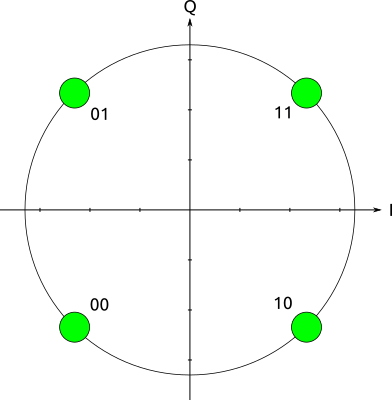
\includegraphics[width=1\linewidth]{images/theory/qpsk.png} a) \\
    }
    \end{minipage}
    \hfill
    \begin{minipage}[h]{0.43\linewidth}
    \center{
        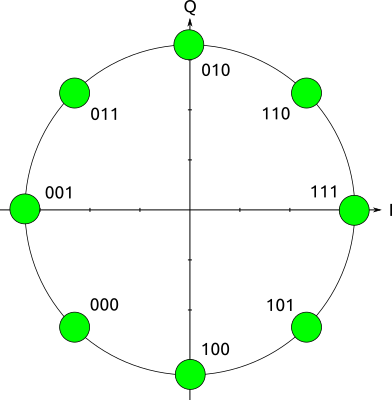
\includegraphics[width=1\linewidth]{images/theory/8psk.png} b) \\
    }
    \end{minipage}
    \vfill
    \begin{minipage}[h]{0.43\linewidth}
    \center{
        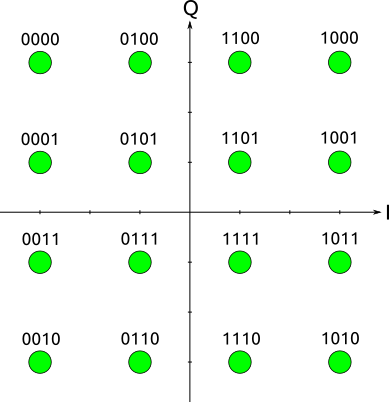
\includegraphics[width=1\linewidth]{images/theory/16qam.png} c) \\
    }
    \end{minipage}
    \hfill
    \begin{minipage}[h]{0.43\linewidth}
    \center{
        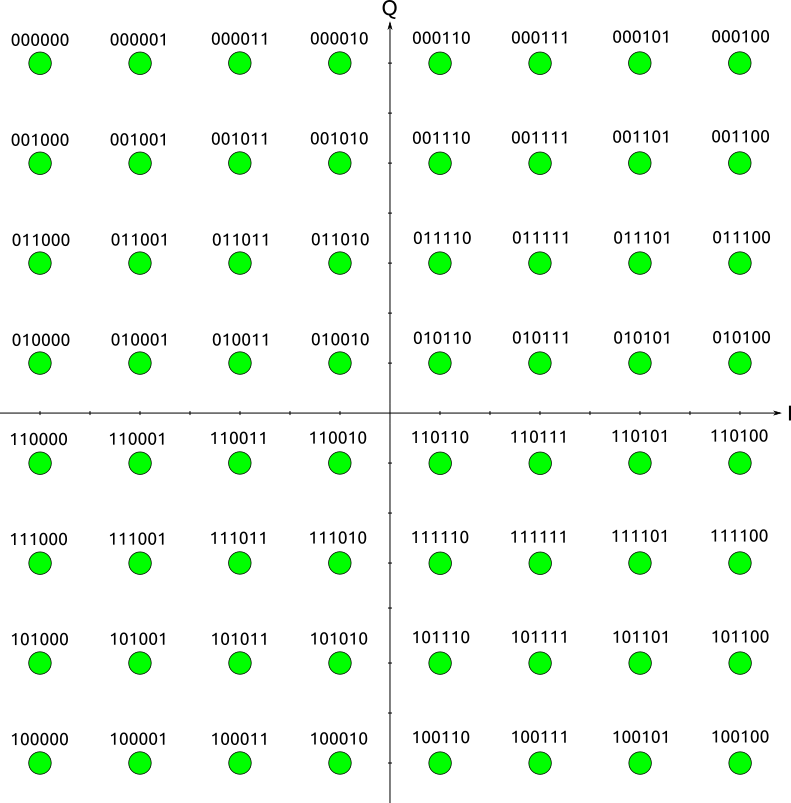
\includegraphics[width=1\linewidth]{images/theory/64qam.png} d)
    }
    \end{minipage}
    \caption{Constellation diagrams for (a) \acrshort{qpsk}, (b) 8-\acrshort{psk}, (c) 16-\acrshort{qam} and (d) 64-\acrshort{qam}.}
    \label{fig:constil}
\end{figure}

In \acrshort{qam}, data is represented by a constellation diagram, where each point on the constellation corresponds to a unique symbol. The position of each point is determined by both its amplitude and phase, allowing for the encoding of multiple bits per symbol. Examples of constellation diagrams used in the work are presented in Fig.~\ref{fig:constil}. For instance, in 16-\acrshort{qam}, the constellation diagram consists of 16 distinct points arranged in a square grid, allowing for the transmission of 4 bits per symbol. The decoding process in the receiver involves identifying the closest constellation point to the received signal, from which the encoded bits are then retrieved. The choice of \acrshort{qam} as a modulation format strikes a balance between the data rate, spectral efficiency, and system robustness, making it a compelling choice for high-speed optical communication systems.

\subsection{Performance Metrics in Optical Communication Systems}


In optical communication systems, evaluating the performance and reliability of data transmission is crucial. Prominent metrics such as \gls{ber}, \gls{evm}, and \gls{mi} are employed for this purpose. Here's an overview of these metrics:

\subsubsection{Bit Error Rate (BER)}
\acrfull{ber} is a pivotal metric that quantifies the number of bit errors (incorrectly received bits) per unit time. It's a direct indicator of the system's error performance.

\begin{equation}
\text{BER} = \frac{\text{Number of bit errors}}{\text{Total number of bits transmitted}}
\end{equation}

The measured (or estimated) \acrshort{ber} is usually converted to an equivalent Gaussian noise Q-factor in $\mathrm{dB}$ using the expression:
\begin{equation}
Q_{\mathrm{BER}}=20 \cdot \log _{10}\left(\sqrt{2} \operatorname{erfc}^{-1}(2 \mathrm{BER})\right),
\end{equation}
where $\operatorname{erfc}^{-1}$ is the inverse complementary error function. This sets the reference Q-factor used in the following evaluation of different indirect methods.

\subsubsection{Error Vector Magnitude (EVM)}
\acrfull{evm} serves as a measure of modulation quality and error performance. It appose the ideal symbol points to the actual symbol points received, providing insight into the distortion induced during transmission.

\begin{equation}
\text{EVM} = \sqrt{\frac{\sum \left(\text{Ideal symbol point} - \text{Received symbol point}\right)^2}{\sum \left(\text{Ideal symbol point}\right)^2}}
\end{equation}

In an optical communication system with \Gls{qam} format, constellation points represented by complex points. $\mathrm{EVM}$ is determined by the formula
\begin{equation}
    \mathrm{EVM}_{m} = \frac{\sigma_{\mathrm{err}}}{|E_{t,m}|} {,} \
    \sigma_{\mathrm{err}}^2 = \frac{1}{I} \sum_{i=1}^{I} |E_{\mathrm{err},i}|^2 {,} \
    E_{\mathrm{err},i} = E_{r,i} - E_{t,i} {.}
\end{equation}
where the propagated vector $E_{r}$ deviates by the vector $E_{\mathrm{err}}$ from the ideally transmitted vector $E_{t}$, and $\mathrm{BER}$ is connected with $\mathrm{EVM}$ as
\begin{equation}
    \mathrm{BER} \approx \frac{(1 - L^{-1})}{\log_2 L}
        \mathrm{erfc}\bigg[ \sqrt{\frac{3 \log_2 L}{(L^2 - 1)} 
        \frac{1}{(k \mathrm{EVM}_{m})^2 \log_2 M}} \bigg] {.}
\end{equation}
In the formula $L$ is the number of signal levels that are identical in each dimension of the constellation, $\log_2 M$ is the number of bits encoded in each \Gls{qam} symbol. More information about these parameters can be found in~\cite{schmogrow}.

% $Q^2$-factor is connected to $\mathrm{EVM}$ as $Q^2 = 1 / \mathrm{EVM}^2$. We will use this definition in the future to assess the quality of the transmission system. The maximum of $Q^2$ factor corresponds to the most optimal transmission parameters.


\subsubsection{Mutual Information}
\gls{mi} assesses the amount of information shared between the transmitted and received signals. It's a measure of the system's capacity to convey information reliably.

\begin{equation}
\text{MI} = \sum_{x \in X} \sum_{y \in Y} p(x, y) \log_2\left(\frac{p(x, y)}{p(x)p(y)}\right)
\end{equation}

where \( p(x, y) \) is the joint probability distribution of the transmitted signal \( x \) and the received signal \( y \), and \( p(x) \) and \( p(y) \) are the marginal probability distributions of \( x \) and \( y \) respectively. In our scenario, 
\( x \) and \( y \) can be construed as the transmitted and received symbols or bits, respectively, and the probability distribution can be ascertained numerically.

These metrics collectively offer a comprehensive understanding of the system's error performance, modulation quality, and information transmission capacity, serving as vital tools for system analysis and optimization.




% 2.2.2 Data-aided EVM

% In an optical communication system with QPSK modulation format, the complex amplitude of this field can be described by 4 points in a complex constellation plane. At the receiver, the received signal vector $\mathbf{E}_r$ deviates by an error vector $\mathbf{E}_{e r r}$ from the ideal transmitted vector $\mathbf{E}_t$ as shown in Fig. 2.1. The data-aided EVM is defined by a root mean square of $\mathbf{E}_{e r r}$ and embraces all (linear and nonlinear) impairments [21]:
% $$
% EVM_m=\frac{\sigma_{e r r}}{\left|E_{t, m}\right|}, \sigma_{e r r}^2=\left\langle\left|\mathbf{E}_{e r r, i}\right|^2\right\rangle, \mathbf{E}_{e r r, i}=\mathbf{E}_{r, i}-\mathbf{E}_{t, i}
% $$
% where $\langle\cdot\rangle$ stands for the averaging operation, $\mathbf{E}_{t, m}$ is the longest ideal constellation vector, serving for normalization.

% By applying the definition 2.2, the EVM in QPSK CO-OFDM transmissions can be calculated as:
% $$
% E V M=\frac{\sqrt{\left\langle\left|c_k-c_{k, \text { ideal }}\right|^2\right\rangle}}{\left|c_{\text {ideal }}\right|},
% $$
% where $c_k$ is the kth received symbol and $c_{k, \text { ideal }}$ is the corresponding ideal constellation point. For a QPSK system with AGWN channel the BER can be estimated from the EVM
% 46

% Figure 2.1: Constellation diagram and error vector for a QPSK signal. Vector $\mathbf{E}_{t, i}$ is the transmitted signal, vector $\mathbf{E}_{r, i}$ is the received signal and $\mathbf{E}_{e r r, i}=\mathbf{E}_{r, i}-\mathbf{E}_{t, i}$ is the error vector
% as [22]:
% $$
% B E R=0.5 \cdot \operatorname{erfc}\left(\frac{E V M^{-1}}{\sqrt{2}}\right)
% $$

% By substituting 2.4 into 2.1, the equivalent Q-factor in $\mathrm{dB}$ can be defined knowing the EVM as:
% $$
% Q_{E V M}=-20 \log _{10}(E V M)
% $$






\section{Signal Formats}
\label{sec:signals}

\subsection{Wavelength Division Multiplexing}
\acrfull{wdm} is a pivotal technology in optical communications, enabling the simultaneous transmission of multiple signals along the same fiber-optic cable, each at a unique wavelength. This effectively multiplies the capacity of the channel, making efficient use of the available bandwidth.

The optical signal  for \Gls{wdm} transmission is represented as a superposition of modulated signals, each associated with a distinct wavelength or frequency. The expression for 
$A(t)$ is given by:
\begin{equation}
A(t)=\sqrt{P_0} \sum_{k=1}^K \sum_{n=1}^{N_{ch}}  c_{kn}   f(t-kT)  e^{-i 2 \pi f_n t},
\label{eq:wdm_nlse}
\end{equation}
where $N_{ch}$ is the number of considered spectral channels, $K$ -- number of symbols in signal, $P_0$ is a average signal power per spectral channel, $f_n=\left(n - \frac{N_{ch}+1}{2}\right) \cdot \Delta$, and $\Delta$ is the channel spacing; $c_{k,n}$ is the complex point from modulation constellation (symbol) of the $k$th symbol on the $n$th channel, $f(t-kT)$ -- pulse shape.

For a system with two polarizations, the optical signal is represented as two separate components $A_x(t)$ and $A_y(t)$:
\begin{eqnarray}
A_x(t)=\sqrt{\frac{P_0}{2}} \sum_{k=1}^K \sum_{n=1}^{N_{ch}}  c_{kn,x} f(t-kT)  e^{-i 2 \pi f_n t}, \nonumber \\
A_y(t)=\sqrt{\frac{P_0}{2}} \sum_{k=1}^K \sum_{n=1}^{N_{ch}}  c_{kn,y} f(t-kT)  e^{-i 2 \pi f_n t}, 
\label{eq:wdm_manakov}
\end{eqnarray}
where $c_{kn,x}$ and $c_{kn,y}$ are the complex constellation points of the 
$k$th symbol on the 
$n$th channel for the $x$ and $y$ polarizations, respectively.
In this work we always suppose that number of symbols and number of \acrshort{wdm} channels for each polarisation are the same. 


% \begin{equation}
% A(z, t) \to \frac{\partial A }{\partial z} = - \frac{\alpha}{2} A - i \frac{\beta_2}{2} \frac{\partial^2 A}{\partial t^2} + i \gamma |A|^2 A.
% \end{equation}

At the receiver, the received signal $A_{out}(t)$ is demodulated to extract the transmitted symbols. The demodulation process can be represented by the following expression:
\begin{equation}
b_k = \int^{\infty}_{\infty} dt A_{out}(t) f^{*}(t - kT),
\label{eq:wdm_matched_filter}
\end{equation}
where $b_k$ is the demodulated symbol, $f^{*}(t - kT)$ is the complex conjugate of the pulse shape. In the scenario involving two polarizations, \( A_{out}(t) \) will be represented as \( A_{out,x}(t) \) and \( A_{out,y}(t) \) for each polarization, leading to the derivation of \( b_{k,x} \) and \( b_{k,y} \) respectively.


The matched filter is an essential component in digital communication systems, utilized at the receiver to maximize the \gls{snr} for a given received signal, thereby facilitating optimal symbol detection. The impulse response of a matched filter is crafted to be a time-reversed and conjugated version of the transmitted signal's waveform. In mathematical terms, if \( f(t) \) is the transmitted signal waveform, the impulse response \( h(t) \) of the matched filter is given by \( h(t) = f^*(-t) \), where \( * \) denotes complex conjugation.

When the received signal traverses the matched filter, the output at the sampling instant yields the optimal \Gls{snr}, making it simpler to detect the transmitted symbols amidst noise. The employment of a matched filter is particularly beneficial in environments laden with significant noise and interference, as it markedly enhances the reliability of symbol detection.
In our case we have time symmetry and always $f(t) = f(-t)$. So Eq.~(\ref{eq:wdm_matched_filter}) represents matched filter for \acrshort{wdm} receiver.

Note that the integral in Eq.~(\ref{eq:wdm_matched_filter}) represents the convolution of the output signal with the function \(f^{*}\). A similar integral expression, albeit in discrete form, can be observed in Eqs.~(\ref{eq:wdm_nlse}) and~(\ref{eq:wdm_manakov}). The summation \(\sum_{n=1}^{N_{ch}}  c_{kn}   f(t-kT)\) serves as a discrete analog of the convolution operation between the discrete points \(c_{kn}\) and the function \(f(t)\). This characteristic is leveraged for practical implementation, aiding in efficient GPU acceleration for numerical simulations, which will be elaborated upon in Chapter~\ref{ch:hpcom}.

\subsubsection{Carrier Pulse}
The choice of carrier pulse shape is crucial as it greatly influences the system's performance, particularly regarding bandwidth efficiency and inter-symbol interference.

A common choice for the carrier pulse in \acrshort{wdm} systems is the Gaussian pulse, valued for its spectral efficiency and simplicity. The Gaussian pulse has a continuous waveform, with its shape defined by the Gaussian function. Another alternative could be the \gls{rc} or \gls{rrc} pulses, frequently chosen due to their ability to control bandwidth and minimize inter-symbol interference.

The choice between \Gls{rrc} and \Gls{rc} filters is driven by the specific requirements of a communication system. However, there are particular advantages associated with the \Gls{rrc} filter which often make it a preferred choice over the \Gls{rc} filter. One of the advantages is the pulse shaping and matched filtering. While the \Gls{rc} filter can be used for pulse shaping at the transmitter or receiver, the \Gls{rrc} filter is designed to be used both at the transmitter and the receiver. When an \Gls{rrc} filter is used at both ends, the combined response is a Raised Cosine filter, which provides optimal \acrshort{isi} mitigation. This split of filtering responsibility between the transmitter and receiver can simplify the design and implementation of the filtering process.

% TODO: check forms

Without loss of generality in this thesis, we consider the following different \acrfull{rz} carrier functions. First example is the function which has cosine slopes and flat central part:
\begin{equation}
    f(t)=
    \left\{
        \begin{aligned}
        \frac{1}{2}\left[1 - \cos\left(\frac{4\pi t}{T}\right)\right] {,} & \; \; 0 \le t \le \frac{T}{4} \; \; \text{or} \; \; \frac{3T}{4} \le t \le T \\
        1 {,} & \; \; \frac{T}{4} < t < \frac{3T}{4} \\
        \end{aligned}
    \right.
    \label{eq:wdm_carrier}
\end{equation}
where {T} is symbol interval.

As a carrier function, one can also use other \acrshort{rz} functions, for example one period of cosine function, which shifted to make overall function positive on the time interval.
\begin{equation}
    f(t)=
    \frac{1}{2}\left[1 - \cos\left(\frac{2\pi t}{T}\right)\right] {,} \; \; 0 \le t \le T {,} 
    \label{eq:wdm_carrier2}
\end{equation}



\begin{figure}[tpb]
    \begin{minipage}[h]{0.3\linewidth}
    \center{
        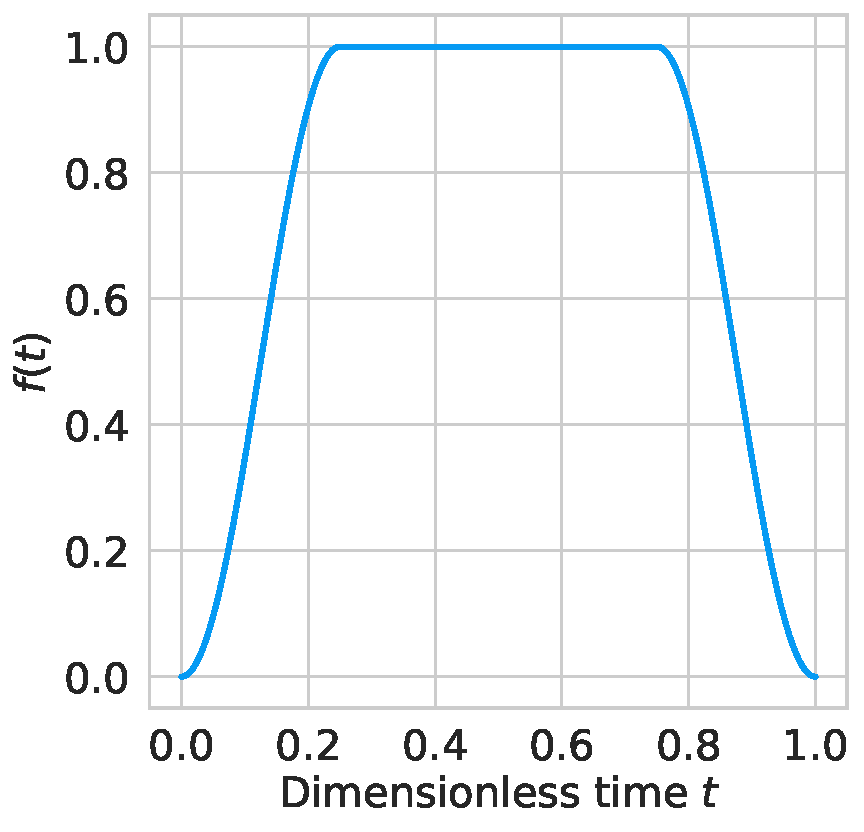
\includegraphics[width=1\linewidth]{images/theory/fat_snake.pdf} (a)
    }
    \end{minipage}
    \hfill
    \begin{minipage}[h]{0.55\linewidth}
    \center{
        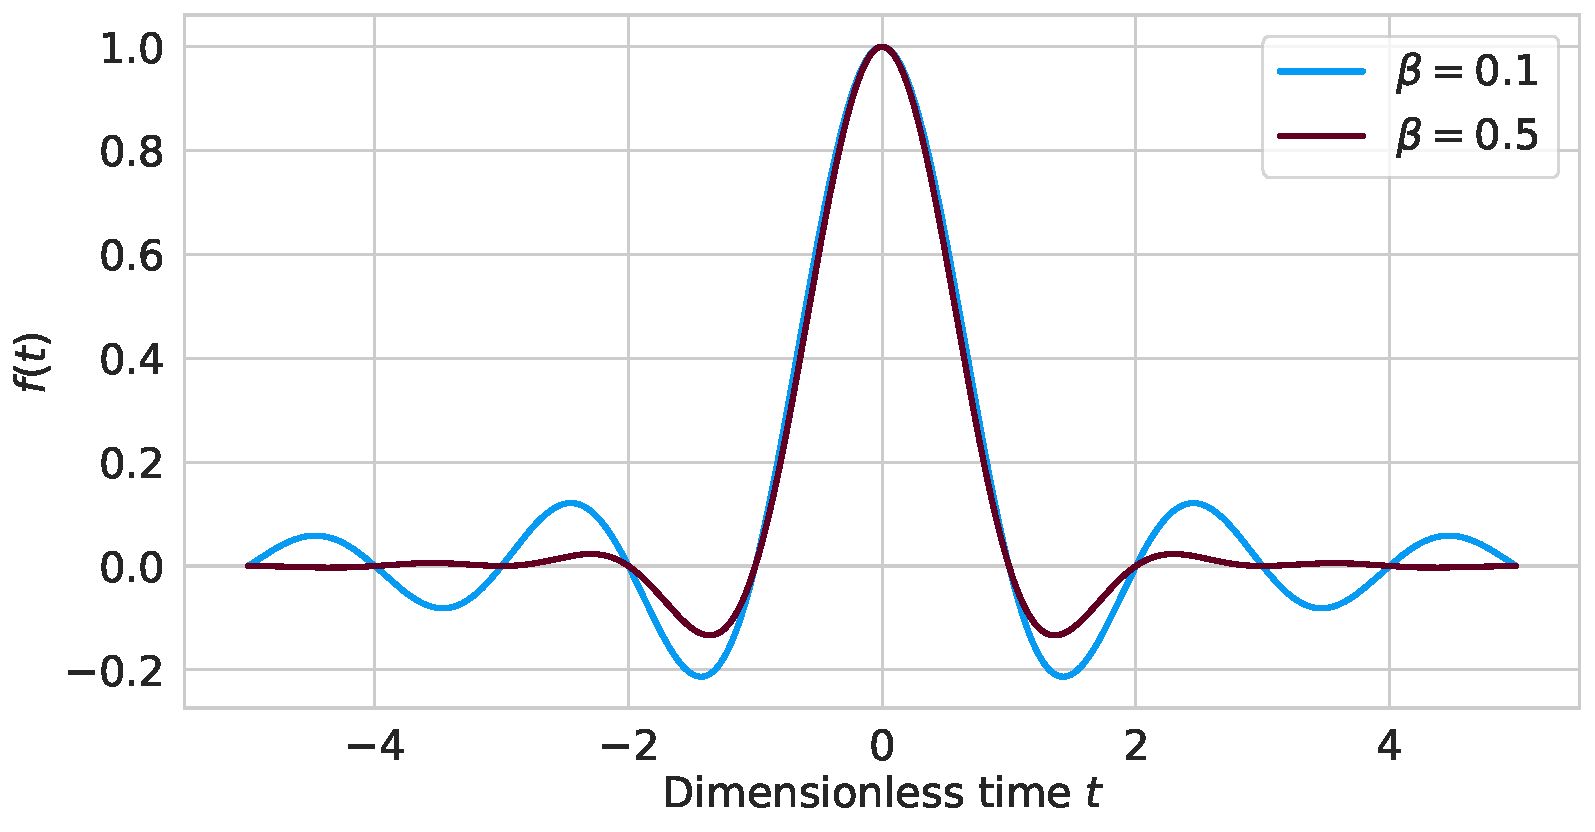
\includegraphics[width=1\linewidth]{images/theory/rc.pdf} (c)
    }
    \end{minipage}

    \begin{minipage}[h]{0.3\linewidth}
    \center{
        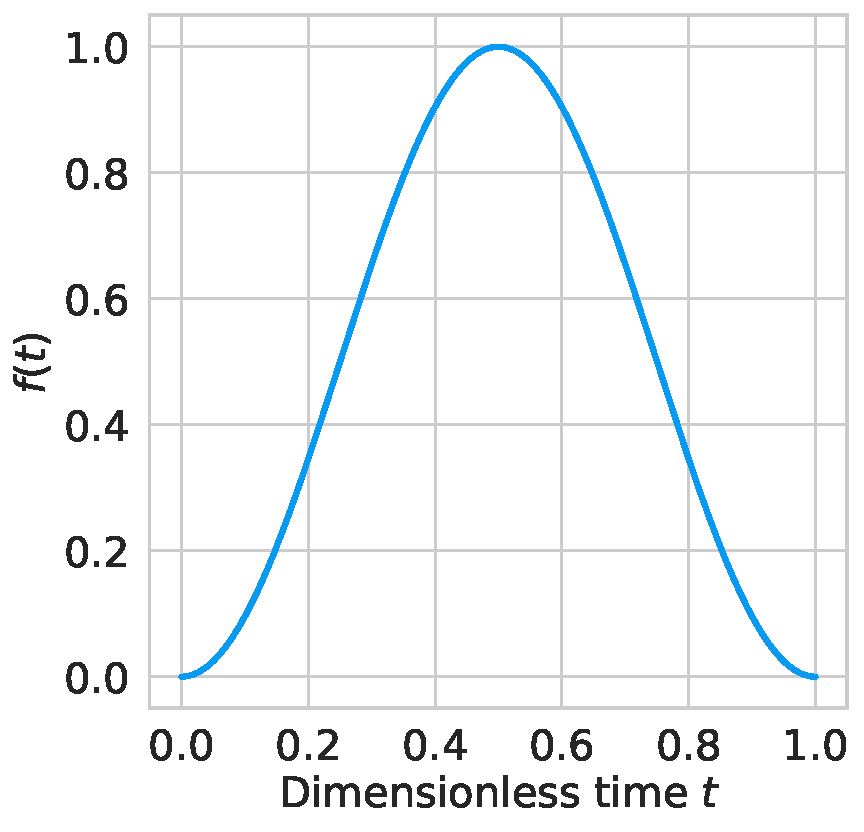
\includegraphics[width=1\linewidth]{images/theory/snake.pdf} (b)
    }
    \end{minipage}
    \hfill
    \begin{minipage}[h]{0.55\linewidth}
    \center{
        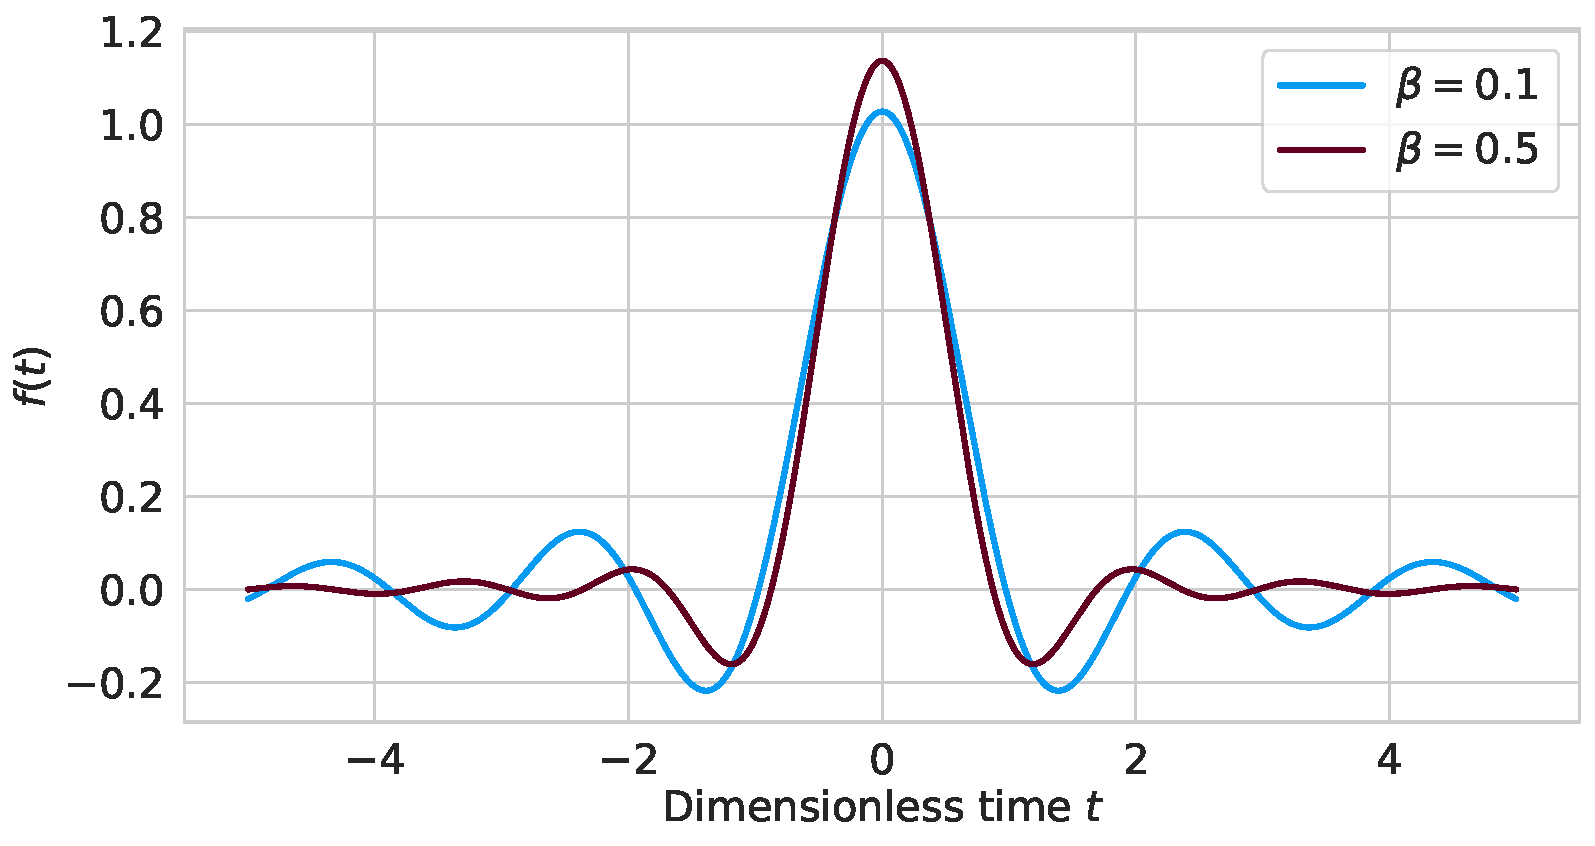
\includegraphics[width=1\linewidth]{images/theory/rrc.pdf} (d)
    }
    \end{minipage}
    \caption{Examples of carrier functions for \acrshort{wdm} signal. \textbf{(a)} function for Eq.~(\ref{eq:wdm_carrier}), \textbf{(b)} function for Eq.~(\ref{eq:wdm_carrier2}), \textbf{(c)} function for \gls{rc} (Eq.~(\ref{eq:rc_time})) and \textbf{(d)} for \gls{rrc} (Eq.~(\ref{eq:rc_time}).}
    \label{fig:f_shapes}
\end{figure}


As we mentioned above, one of the most common choice is \Gls{rc} waveform function. In time space, it is expressed as follows:
\begin{equation}
    f(t) = 
\begin{cases} 
\frac{\pi}{4T} \sinc \left( \frac{1}{2\beta} \right), & t = \pm \frac{T}{2\beta}, \\
\frac{1}{T} \sinc \left( \frac{t}{T} \right) \frac{\cos\left( \frac{\pi \beta t}{T} \right)}{1 - \left( \frac{2\beta t}{T} \right)^2}, & \text{otherwise}.
\end{cases}
\label{eq:rc_time}
\end{equation}
And other is \Gls{rrc} with a roll-off factor $\beta$:
\begin{equation}
    f(t) = \begin{cases}
    \frac{1}{T}\left( 1 + \beta \left( \frac{4}{\pi} - 1 \right) \right),& t = 0, \\
    \frac{\beta}{T \sqrt{2}} \left( \left( 1 + \frac{2}{\pi} \right) \sin\left( \frac{\pi}{4\beta} \right) + \left( 1 - \frac{2}{\pi} \right) \cos \left( \frac{\pi}{4\beta} \right) \right),& t = \pm \frac{T}{4 \beta},\\
    \frac{1}{T} \frac{\sin \left( \pi \frac{t}{T} \left( 1 - \beta \right) \right) + 4 \beta \frac{t}{T} \cos \left( \pi \frac{t}{T} \left( 1 + \beta \right) \right)}{\pi \frac{t}{T} \left( 1 - \left( 4\beta \frac{t}{T} \right)^2 \right)},&\text{otherwise}.
    \end{cases}
\label{eq:rrc_time}
\end{equation}

All waveforms are represented in Fig.~\ref{fig:f_shapes}.
For \Gls{nft} analysis, we will focus on the study of symbols with a carrier function in the form~(\ref{eq:wdm_carrier}). And for \gls{wdm} signal analysis we will use \gls{rrc}~(\ref{eq:wdm_carrier}) (as we are interested in real systems).




\subsection{
Orthogonal Frequency-Division Multiplexing
}
\label{sec:ofdm}

\gls{ofdm} signal combines modulation and multiplexing. To form a symbol, the term "subcarrier"\ is used, which in fact is one of the Fourier harmonics in the frequency space from which the signal is formed. One isolated symbol on a time slot of $ T $ is the sum of independent subcarriers modulated according to the chosen modulation type:
\begin{equation}
    A_{\text{symb}}(t) = \sum_{k=0}^{N-1} c_k e^{i \frac{2 \pi k}{T} t} {,}
    \label{eq:ofdm_symbol}
\end{equation}
where $N$ -- number of subcarriers,
$T$ -- symbol duration,
$c_k$ -- modulated data. 
Depending on the modulation type, the corresponding constellation diagram is selected (Fig.~\ref{fig:constil}).

In practice, the number of subcarriers is chosen as $N = 2^p$ ($p$ is a positive integer) in order to use the \gls{fft} algorithms. 
% The scheme of forming the OFDM signal is shown in Fig.~\ref{fig:ofdm}. 
The input is serial data which is divided into $N$ parallel threads. Each data stream is encoded according to the selected modulation format (\acrshort{qpsk} or \acrshort{qam}). Each individual stream corresponds to a specific frequency, and the encoded data determines the complex amplitude for that frequency. Thus obtained N numbers are used further in the \Gls{fft}, the result of which is the one \acrshort{ofdm} symbol. 

% \begin{figure}[htpb]
%     \center{
%         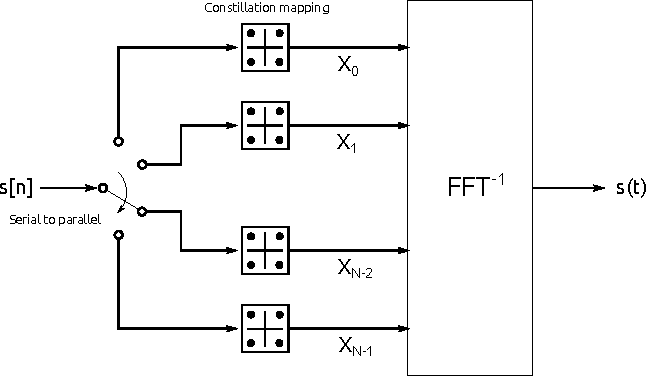
\includegraphics[width=0.7\linewidth]{images/theory/ofdm.pdf}
%     }
%     \caption{OFDM signal generation}
%     \label{fig:ofdm}
% \end{figure}

\acrfull{ofdm} signal generation in a practical scenario encompasses multiple symbols, a guard interval, and a cyclic prefix to mitigate \acrfull{isi} and ensure seamless reception. 
When transmitting multiple \acrshort{ofdm} symbols, the signal \( A(t) \) over multiple symbol intervals is represented as a sum over all symbols \( K \) and all sub-carriers \( N \) as follows:
\begin{equation}
A(t) = \sum_{k=0}^{K-1} \sum_{n=0}^{N-1} c_{kn} \cdot e^{i \frac{2 \pi k}{T} (t - kT)}
\label{eq:ofdm_signal}
\end{equation}
where\( K \) is the total number of \acrshort{ofdm} symbols, \( T \) is the symbol duration.

A cyclic prefix is a portion of the \acrshort{ofdm} symbol copied and prepended to the symbol to combat \acrshort{isi}. If the cyclic prefix duration is \( T_{\text{CP}} \), the signal with the cyclic prefix \( A_{\text{CP}}(t) \) is given by:
\begin{equation}
A_{\text{CP}}(t) = 
\begin{cases} 
A(t - (T + T_{\text{CP}})k + T_{\text{CP}}), & \text{for } kT \leq t < kT + T_{\text{CP}} \\
A(t - k(T + T_{\text{CP}})), & \text{for } kT + T_{\text{CP}} \leq t < (k+1)T + kT_{\text{CP}}
\end{cases}
\end{equation}

\begin{figure}[htpb]
    \center{
        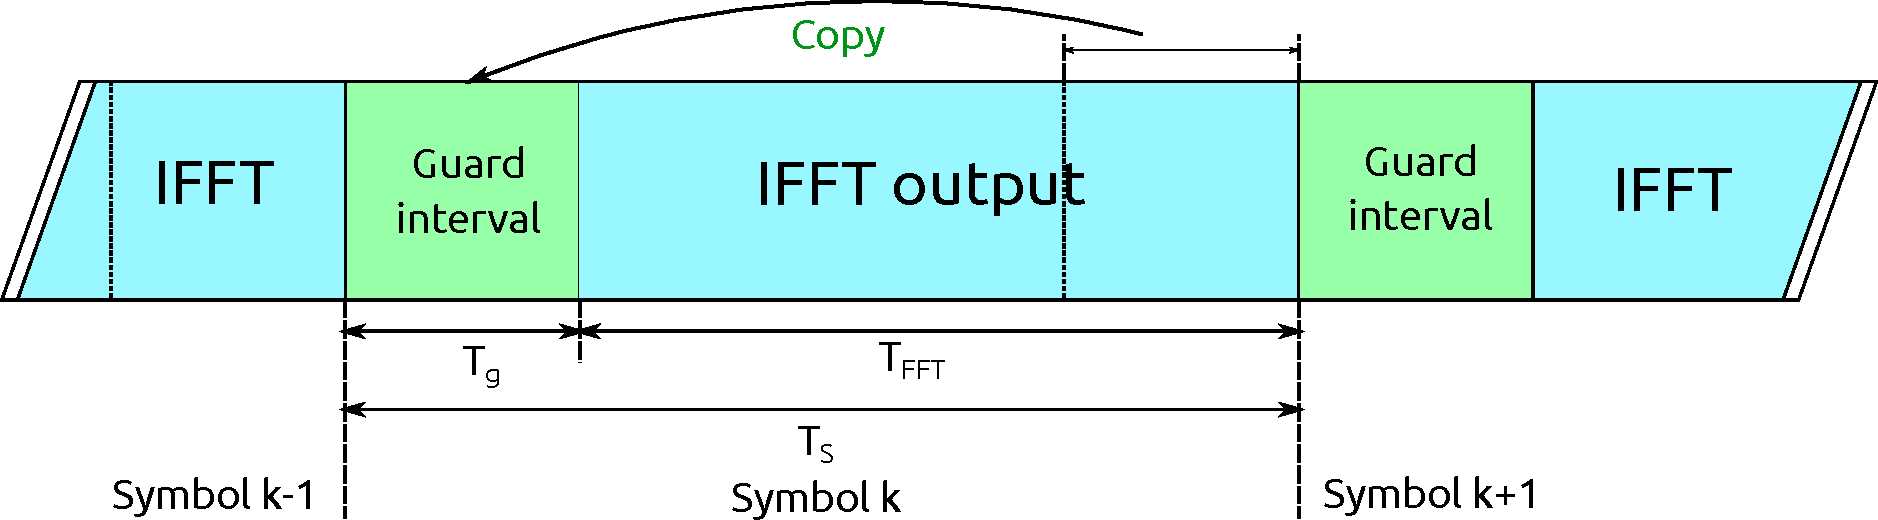
\includegraphics[width=0.9\linewidth]{images/theory/ofdm_scheme.pdf}
    }
    \caption{Addition of a guard period to an \acrshort{ofdm} signal}
    \label{fig:ofdm_signal}
\end{figure}

A guard interval is added between \acrshort{ofdm} symbols to prevent inter-symbol interference. The guard interval duration is typically equal to the cyclic prefix duration \( T_{\text{CP}} \).
The resulting signal \( A_{\text{final}}(t) \) which includes multiple symbols, the cyclic prefix, and the guard interval is thus represented by the formula for \( A_{\text{CP}}(t) \) over the entire transmission duration (Fig.~\ref{fig:ofdm_signal}). Within the scope of this work, the cycle prefix will not be incorporated into the \Gls{ofdm} signals. Instead, Eq.~(\ref{eq:ofdm_signal}) or Eq.~(\ref{eq:ofdm_symbol}) will be used as references.


To decode a signal, the procedure is performed in the reverse order.
The cyclic prefix appended to each \acrshort{ofdm} symbol is removed. 
Once the cyclic prefix is removed, the receiver performs a \Gls{fft} on each \acrshort{ofdm} symbol to convert it from the time domain to the frequency domain. The \Gls{fft} operation segregates the aggregated \acrshort{ofdm} symbol back into its constituent subcarriers. This transformation is the reverse of what was done at the transmitter during the \Gls{ifft} operation. Following the \Gls{fft}, each sub-carrier is individually demodulated to extract the data bits. The demodulation is performed based on the modulation scheme used at the transmitter, for example, \acrshort{qam} or \acrshort{psk}. The data from all sub-carriers is then aggregated to form the complete data stream.